\section{A possibility worth constructing}
The grand mandate is to discover a consequential opportunity, construct the missing means, deliver a useful outcome, and test whether the resulting enterprise can equip a more capable successor. The productive opening investigated here is \emph{custom measurement capacity}: a scientific team should be able to state a precise event relationship and obtain a transferable digital instrument that implements it, with acceptance evidence another engineer can inspect.

Consider an experiment that produces four event channels. A herald $A$ opens an opportunity; a probe $B$ must follow within a specified interval; a confirmation $C$ must follow the probe; and a veto arriving later must still cancel the decision. A second experiment on the same interface must remain independent. The question is sufficiently concrete to be executable, yet it matters to an experimenter's ability to define what gets measured or acted upon. Incorrect cross-triggering, premature acceptance or ambiguous simultaneous-event behavior changes the measurement itself.

This use case is an application hypothesis, not a recovered customer order. The initial beneficiary is a small instrumentation OEM or experimental photonics team that already has a digitized event interface and needs a custom, bounded logical kernel. EventWeaver does not supply a time-to-digital converter, optical detector, calibrated clock, timestamp parser or physical feedback path. The first commercial acceptance is acceptance of a \emph{firmware design pack}; board deployment requires another contract and evidence gate.

\begin{table}[htbp]
\centering\small
\begin{tabular}{L{0.13\textwidth}L{0.80\textwidth}}
\toprule
Before & Built-in filtering may not express independent, multistage, delayed-veto predicates. A buyer can use custom software or HDL, but must specify, implement and verify the behavior.\\
Construction & A contract validator, an age-indexed event compiler, executable models, emitted Verilog, independent conventional RTL, an offline oracle and an acceptance harness.\\
After & A valid eight-channel contract produces a replayable, synthesizable kernel with explicit endpoint, overlap, reset and group semantics.\\
Value & Less bespoke construction may be required for a supported class, and acceptance becomes reproducible. The amount a buyer would pay for this reduction remains unmeasured.\\
Next & A new network grammar makes one accepted instrument decision an input to a later instrument, while reusing unchanged kernels.\\
\bottomrule
\end{tabular}
\caption{The before-and-after claim is specific to this constructed delivery route. Conventional custom development remains a feasible alternative.}
\end{table}

\subsection{The first beneficiary experience}
The beneficiary supplies a JSON specification and clocked event masks. In the demonstration, the first group uses channels 0--3, the second channels 4--7. The first group permits $A$--$B$ lags of one to three ticks and $B$--$C$ lags of one to two ticks, with a decision seven ticks after the anchor. The second group uses different bounds and an eight-tick deadline.

The system rejects unsupported requests before generation. It then emits a readable intermediate representation, a Python execution model, C++ and Verilog, and a manifest binding the deliverable to the specification. A buyer can replay the included trace, inspect every output, run the independent verifier, or use the browser edition to insert a late veto and observe the changed decision. A veto at the decision tick cancels the affected group; the other group's decision remains intact. Reset clears pending anchors. Repeated anchors overlap without becoming one shared state machine.

An acceptance failure produces a counterexample, a refusal or a bounded correction under the original contract. It does not produce an automatically weakened specification. This distinction is part of the product: a verified answer to the wrong event semantics would still be an unsuccessful measurement instrument.

\begin{figure}[htbp]
\centering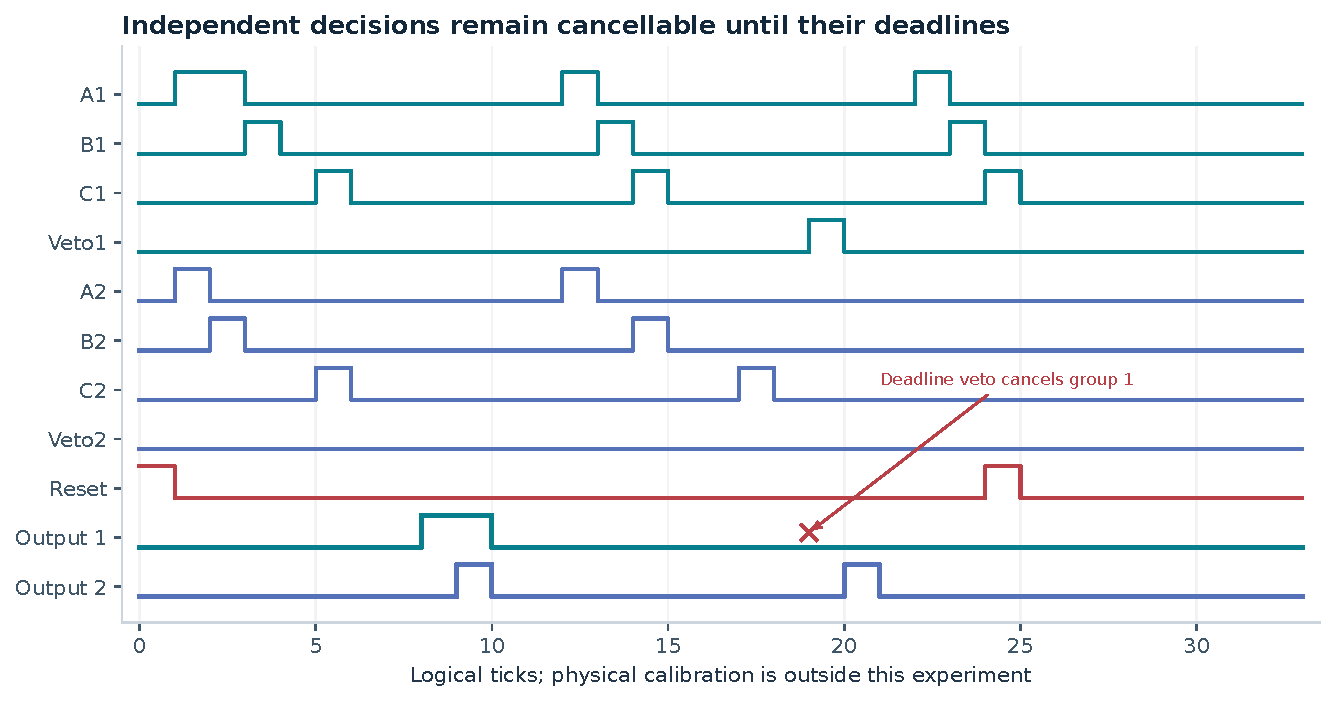
\includegraphics[width=\textwidth]{figures/event_trace.pdf}
\caption{Executed 34-tick demonstration. Group 1 accepts at ticks 8 and 9. Both groups fire at tick 9. A later endpoint veto cancels group 1 at tick 19 while group 2 still accepts at tick 20. Reset at tick 24 clears another pending anchor. Ticks are logical bins, with no physical timing claim.}
\end{figure}

\subsection{The four questions are different}
The campaign asks four questions separately. Does the useful digital capability work? Yes, within the tested contract and bounded proof scope. Can this service sustain a complete enterprise? The selected model says no. Does expert agent operation establish an exclusive advantage? No: the competent conventional control ties functionally and its Python model is faster. Does retained capability help a fresh mission after costs? It provides a working starting point for the network extension, but the identical-library control ties and the US\$4,100 extension is an additional research cost. Those answers can coexist without converting a correct prototype into a fictional breakthrough.

\section{The frontier moved; the commercial bridge still had to be built}
The frontier investigation began with the four requested OpenAI sources, then examined other laboratories and open-source methods. Exact releases were verified before use. The source register distinguishes availability, actual access, limitations and the smallest commercial test for each material advance.

OpenAI's October 6 mathematical collection supplies candidate results and formalization artifacts produced by an internal model; the study did not have that model or reproduce its proof corpus. The October 26 academic-community announcement treats the materials as research inputs and explicitly leaves practical algorithmic consequences for further work. We therefore did not assume a new commercial SAT algorithm from an announcement. The collection was pinned at commit \texttt{7ef5c0cc}; its history also preserves withdrawals and revisions, making version and failure custody part of the investigation.\cite{math,academic,mathrepo}

GPT-6 Astra was released September 3, 2026, and GPT-6.1 Terra October 26. Published standard API prices are respectively US\$10/50 and US\$1/5 per million input/output tokens; Terra cached input is US\$0.05 per million. These prices suggest routing routine intake to a cheaper model and difficult specification work to a stronger one. The session used available Astra agents; Terra was verified in the catalog but not separately benchmarked. No checkpoint identifier or per-task invoice was exposed.\cite{astra,terra,changelog}

\begin{longtable}{L{0.18\textwidth}L{0.22\textwidth}L{0.25\textwidth}L{0.26\textwidth}}
\caption{Frontier register: what changed, what was accessible, and the test needed to make it commercially relevant.}\label{tab:frontier}\\
\toprule Advance / date & Demonstrated or reported capability & Access and limitation in this study & Smallest commercial test \\
\midrule\endfirsthead
\toprule Advance / date & Capability & Access / limit & Commercial test \\
\midrule\endhead
OpenAI math, Oct. 6; collection pinned Oct. 26 & Public manuscripts and some formal proofs at mixed verification stages & Artifacts read; internal generator unavailable; no proof-corpus rerun & Extract one applicable construction and beat a mature finite-instance baseline.\\
Academic communities, Oct. 26 & Public math/CS materials and an external understanding program & Research announcements; physics materials not accessed & Demonstrate a usable algorithm under its exact hypotheses.\\
GPT-6.1 Terra, Oct. 26 & Provider-reported gains in visual reasoning, computer use and cost efficiency & Public release; catalog-listed here, not experimentally compared & Compare cost per accepted intake task, including escalation and repair.\\
GPT-6 Astra, Sept. 3 & Tool-using reasoning, coding and scientific work & Available authoring family; immutable model checkpoint and billing unavailable & Construct the instrument and subject it to independent checks.\\
AlphaEvolve, updated primary report & Evaluator-guided program search across several domains & Public evidence inspected; service not used & A real evaluator must measure the proposed improvement; rivals receive improving AI too.\\
OpenEvolve and formal tools & Open implementations of evaluator-driven search and deterministic verification & Sources examined; standard compiler and Yosys used here & Retain a reproducible executable, not an unsupported model judgment.\\
YoWASP Yosys 0.70, Oct. 13 & Locally executable HDL synthesis, CXXRTL and SAT tooling & Installed version pinned; actual commands and logs preserved & Synthesize and execute both candidates, then prove their bounded equivalence.\\
\bottomrule
\end{longtable}

The broader search included Anthropic's current model documentation, DeepSeek-Prover-V2, OpenEvolve and HiGHS. None was represented as an execution result in this campaign. Their roles were to challenge the notion that exclusive access to one model could sustain an advantage. The full source matrix preserves access distinctions rather than folding every promising announcement into an assumed production system.\cite{alphaevolve,openevolve,deepseek,yosys}

\subsection{The frontier-crossing account}
\textbf{Previously binding constraint:} an uncommon measurement predicate required bespoke specification, implementation and checking, often alongside an existing acquisition system. \textbf{Recent change:} more capable tool-using models and lower-cost routine operation plausibly reduce parts of that construction burden. \textbf{Missing construction:} a bounded event language, a reusable implementation, independent acceptance checks and a support arrangement. \textbf{Newly deliverable outcome in this study:} an executable, checked digital design pack and a composed successor.

This is a candidate \emph{economic} crossing. It is not evidence that temporal logic became technologically possible in 2026. No controlled old-model/new-model trial was performed, so a measured historical cost reduction cannot be assigned to Terra, Astra or AGI in general. The construction succeeded; the complete-cost commercial test determines whether the proposed crossing is enough.

\subsection{The cost-adjusted operating system}
A production design would use inexpensive extraction and administration, selective stronger-model escalation, and deterministic tools for every acceptance-critical step. Once a request falls inside the frozen grammar, compilation and replay need no frontier-model invocation. The model contributes to discovery, specification, code construction and exceptions; the checker supplies reproducible acceptance evidence.

The US\$25 inference allowance per contracted order is an explicit cost estimate for intake and exception handling. It is not charged per clock tick. Shared model/tool development is charged once, and a common defect creates shared repair costs plus customer-specific obligations. Computer operation was used where helpful for file construction, local compilation and browser QA; it does not demonstrate that the native enterprise runtime or a vendor acquisition board was operated.

\section{Discovery before demonstration}
The opening question was: what valuable possibility is now achievable that existing organizations are not equipped to pursue? The second question was: what could we construct that changes the set of possible valuable activities? Five complementary searches produced a diverse shortlist before the selected compiler was implemented.

\begin{longtable}{L{0.18\textwidth}L{0.36\textwidth}L{0.37\textwidth}}
\caption{Five lenses and the evidence they contributed.}\\
\toprule Lens & Opening & Challenge that changed the decision\\
\midrule\endfirsthead
\toprule Lens & Opening & Challenge\\\midrule\endhead
Unmet needs & Precise independent event relationships that an installed filter does not express & The useful outcome must be a specified digital kernel; a whole calibrated instrument cannot be presumed.\\
New capabilities & Current reasoning/coding plus executable verification could shorten bespoke construction & Provider benchmarks do not establish accepted-outcome economics; production routing remains unmeasured.\\
Unexpected combinations & Open acquisition tools, explicit contracts, independent checking and supported reuse & Competent conventional teams and rivals can assemble the same combination.\\
Missing means & A compiler that preserves overlap, endpoints and late veto, with evidence another engineer can replay & Temporal specification-to-FPGA work already exists; the contribution is this bounded delivery construction.\\
Successor possibilities & A verified output becomes an input to a later instrument, extending the accepted grammar & The extension must actually be built, separately frozen, freshly checked and charged.\\
\bottomrule
\end{longtable}

The candidate families included laboratory protocol generation, private cross-owner cohort/aggregate collaboration, shared assay infrastructure, flexible-load capacity arrangements, material/industrial matching, and custom temporal instruments. Protocol generation faced free capable tools and unperformed wet-lab validation. Private collaboration offered consequential benefits but left institutional participation and data access as the central unexecuted dependencies. Shared assays already had substantial community infrastructure. Flexible-load and industrial routes required site evidence and external authority that a local simulator could not supply.

The temporal instrument was selected for a bounded construction campaign because its essential digital capability could be constructed and falsified here, while its commercial weakness could be exposed without pretending that a physical experiment had happened. Constructibility alone did not earn transformational flagship status. The subsequent conventional tie, removal counterfactual and complete-cost failure rejected that stronger claim. The initial selection record is preserved unchanged; a separately dated return-to-search record documents the rejection and renewed comparison.

\subsection{Prior art narrowed the claim}
NIST already provides open-source FPGA acquisition instruments and explicitly supports custom data collection logic. BrightEyes-TTM supplies an open FPGA time-tagging system that has been used in microscopy. These establish practical alternatives, not empty adjacent categories.\cite{nist,brighteyes}

Swabian's Conditional Filter manual, version 2.22.6.0, documents a specific limitation: two independent trigger/filter groups cannot be configured separately in that built-in filter, and cross-triggering can reduce filtering efficiency. Its raw-stream CustomMeasurement and FPGA Link routes nevertheless support custom work. EventWeaver is not claimed to be physically compatible with them; the vendor interface is a separate integration problem.\cite{conditional,rawstream,fpgalink}

Temporal specification-to-FPGA compilation also predates this edition. RTLola work compiles stream-monitoring specifications into synthesizable VHDL; related temporal monitoring systems provide further prior art. Accordingly, this study does not claim invention of temporal monitoring, a universally novel compiler, or an outcome beyond all human foresight. Its non-obviousness claim is limited to an investigated combination and a narrower commercial hypothesis.\cite{rtlola,r2u2}

\subsection{Continuation and active ownership}
The existing AGI Alpha repository and 717 available comments on issue 4850 were inspected. Active studies covered resilient compute placement, conserved production hypotheses, causal capacity and quantitative microscopy image transfer. The last concerns image/coordinate measurement preservation, rather than photon event logic or RTL. No matching temporal-instrument study was found in the inspected coordination record; that search result is not universal absence.

The campaign is additive to pinned main \texttt{12770c22b4a9f90f2013bbfb64242f912ba5071e}. It preserves the exact prior editions and the existing publication owner. A separate source branch and draft review package do not imply canonical Pages publication, merged software qualification or permission to operate deployed contracts.

\section{Constructing the digital instrument}
\subsection{A precise acceptance semantics}
At each logical clock tick $t$, the input is an eight-bit mask. A bit indicates at least one event in that bin; multiplicity within the bin is not represented. A predicate $j$ specifies distinct channels $A_j,B_j,C_j,V_j$, positive inclusive lag bounds $[l_1,u_1]$ and $[l_2,u_2]$, and a deadline $D_j$, with
\begin{equation}
1\le l_1\le u_1,\quad 1\le l_2\le u_2,\quad u_1+u_2\le D_j\le20.
\end{equation}
The output at $t$ is one exactly when an anchor exists at $t-D_j$, an eligible $B$--$C$ path exists, and no veto occurs from anchor through deadline:
\begin{align}
y_j(t)={}& A_j(t-D_j)\ \wedge\ \neg\bigvee_{k=0}^{D_j}V_j(t-D_j+k)\nonumber\\
&\wedge\bigvee_{a=l_1}^{u_1}\ \bigvee_{b=l_2}^{u_2}
\left[B_j(t-D_j+a)\wedge C_j(t-D_j+a+b)\right].\label{eq:contract}
\end{align}
Synchronous reset dominates the mask and clears every pending state. An output after reset needs a complete new history. Positive lag bounds prevent same-tick $A$--$B$ or $B$--$C$ matching, although unrelated channels can coexist in a sample. Multiple paths for one anchor merge to one Boolean result; repeated anchors remain independent. An empty sample advances time. There is no backpressure, implicit timestamp reordering or silent overflow policy: the buyer must supply a lossless clocked-bin interface.

Up to four predicates are supported. They may intentionally share declared channels, but a predicate never reads another group's undeclared channel. The checker rejects malformed names, ranges, channel identifiers, duplicate names, illegal deadlines and unsupported references before emitting a deliverable.

\subsection{The representation that was built}
The compiler uses age-indexed prefix states: surviving anchors, eligible $A$--$B$ prefixes, and completed paths waiting for their final decision. Veto clears all relevant prefixes. The final state stays cancellable through the endpoint. Boolean OR merges alternative paths, preserving the observable answer without counting the same anchor more than once.

Before synthesis, a predicate uses
\begin{equation}
u_1+(u_1-l_1+1)u_2+D_j-l_1-l_2+1
\end{equation}
Boolean state bits. This is a construction formula, not an optimality theorem. Wide windows can make the prefix representation larger than a direct history representation. The independent implementation instead retains event histories and evaluates Equation~\ref{eq:contract} directly. The mathematical oracle scans the event history independently.

The demonstration kernel synthesized to 29 state bits and 73 generic cells: 29 synchronous-reset flip-flops and 44 logic cells, with no latches or unresolved modules. These are generic Yosys statistics, not FPGA lookup-table utilization, physical silicon area, power or clock frequency. Generated C++ was actually compiled and replayed; emitted RTL was actually executed through CXXRTL.

\subsection{What verification establishes}
The checks compare candidate model, conventional model, independent oracle and actual RTL. Bounded SAT miters use explicit initialization/reset assumptions and recorded depths. They establish equivalence over those bounded traces; they do not constitute a universal proof of every possible grammar instance or analog interface. The recurrence provides a useful invariant argument, but the claim remains tied to executed checks and their limits.

The valuable construction is the complete chain from contract to executable behavior to inspectable evidence. An emitted file alone would not satisfy it. Neither would a simulator that assigned successful delivery without executing the essential digital work.
